\documentclass[11pt]{article}
\usepackage[T1]{fontenc}
\usepackage[utf8]{inputenc}
\usepackage{lmodern}
\usepackage{geometry}
\geometry{margin=1in}
\usepackage{microtype}
\usepackage[colorlinks=true,linkcolor=blue!50!black,citecolor=green!40!black,urlcolor=blue!50!black]{hyperref}
\usepackage{booktabs}
\usepackage{array}
\usepackage{longtable}
\usepackage{amsmath}
\usepackage{amssymb}
\usepackage{amsthm}
\usepackage{tikz}
\usetikzlibrary{arrows.meta,positioning,calc,shapes.geometric,fit}
\usepackage{xcolor}
\usepackage{textcomp}
\usepackage{listings}
\setlength{\emergencystretch}{3em}

% Sanskrit transliteration
\DeclareUnicodeCharacter{1E63}{\d{s}}
\DeclareUnicodeCharacter{1E62}{\d{S}}
\DeclareUnicodeCharacter{1E47}{\d{n}}
\DeclareUnicodeCharacter{1E6D}{\d{t}}
\DeclareUnicodeCharacter{1E0D}{\d{d}}
\DeclareUnicodeCharacter{1E5B}{\d{r}}
\DeclareUnicodeCharacter{1E43}{\d{m}}
\DeclareUnicodeCharacter{1E25}{\d{h}}
\DeclareUnicodeCharacter{1E45}{\.{n}}

\lstdefinelanguage{lean}{
  keywords={theorem, def, inductive, noncomputable, instance, structure,
    abbrev, where, fun, Prop, Type},
  sensitive=true,
  comment=[l]{--},
  morecomment=[s]{/-}{-/},
}
\lstset{
  language=lean,
  basicstyle=\footnotesize\ttfamily,
  keywordstyle=\bfseries,
  commentstyle=\itshape\color{black!60},
  columns=fullflexible,
  keepspaces=true,
  upquote=true,
  frame=leftline,
  framerule=0.6pt,
  rulecolor=\color{black!40},
  xleftmargin=1.2em,
  aboveskip=6pt, belowskip=6pt,
  breaklines=true,
  literate=
    {Φ}{{$\Phi$}}1 {Ψ}{{$\Psi$}}1 {φ}{{$\varphi$}}1 {ψ}{{$\psi$}}1
    {κ}{{$\kappa$}}1 {α}{{$\alpha$}}1 {β}{{$\beta$}}1 {ι}{{$\iota$}}1
    {∀}{{$\forall$}}1 {∃}{{$\exists$}}1 {∈}{{$\in$}}1 {∉}{{$\notin$}}1
    {∪}{{$\cup$}}1 {∩}{{$\cap$}}1 {⋂}{{$\bigcap$}}1 {⊆}{{$\subseteq$}}1
    {∅}{{$\emptyset$}}1 {∧}{{$\wedge$}}1 {∨}{{$\vee$}}1 {¬}{{$\neg$}}1
    {→}{{$\to$}}1 {↔}{{$\leftrightarrow$}}1 {≃}{{$\simeq$}}1
    {⊤}{{$\top$}}1 {⊥}{{$\bot$}}1 {≠}{{$\neq$}}1 {≤}{{$\leq$}}1
    {ᶜ}{{$^{\mathsf c}$}}1 {∼}{{$\sim$}}1 {⟨}{{$\langle$}}1 {⟩}{{$\rangle$}}1
    {ℕ}{{$\mathbb{N}$}}1
}

\newcommand{\code}[1]{\texttt{#1}}
\newcommand{\BE}{\code{BinaryEvidence}}
\newcommand{\lean}[1]{\texttt{\detokenize{#1}}}

\theoremstyle{plain}
\newtheorem{theorem}{Theorem}[section]
\newtheorem{proposition}[theorem]{Proposition}
\theoremstyle{definition}
\newtheorem{definition}[theorem]{Definition}
\newtheorem{remark}[theorem]{Remark}

\title{Formal Buddhist Logic\\[2pt]
\large The catuṣkoṭi, non-perception, valid reasons, exclusion and the two truths,\\
mechanized over PLN evidence}
\author{Oru\v{z}i \and Zarathustra Goertzel}
\date{\today}

\begin{document}
\maketitle

\begin{abstract}
Indian Buddhist logicians drew distinctions, more than a millennium ago, that formal
reasoning systems keep rediscovering under other names: evidence for a claim against
evidence against it; ``no evidence'' against ``evidence of absence''; denying a claim
against asserting its opposite; a concept as what it excludes; conventional truth against
ultimate truth. We give each of these distinctions an exact mathematical reading on
carriers that an existing reasoning library already uses, chiefly the two-channel evidence
of Probabilistic Logic Networks (PLN), and we prove the readings in Lean 4.
The four corners of the catuṣkoṭi are exactly the values that double negation fixes on PLN
evidence, and the logic of supported formulas over that evidence is First Degree
Entailment. Dharmakīrti's rule of non-perception becomes one law with a single side
condition, perceptibility, under which absence of evidence is evidence of absence; eight
results already in the library turn out to be instances of it, among them Chalmers's
``that's all'' clause. The three marks of a valid reason, Dignāga's wheel of reasons, the
apoha theory of meaning by exclusion, which meets the distinction calculus at the sorites, and
Madhyamaka's two truths each receive a theorem
with positive and negative controls. A final section separates thirteen kinds of
``no value'' that programming languages tend to collapse. Every theorem cited is proved
without \code{sorry}, with no axioms beyond Lean's standard three.
\end{abstract}

\tableofcontents

\section{Introduction}

The motivation is semantic clarity. Several techniques familiar from knowledge
representation and automated reasoning, namely local closed-world assumptions, coverage-based
scoring of candidate rules, paraconsistent treatment of conflicting data, and learning
concepts from negative examples, are usually presented separately and justified case by case.
The Buddhist logical tradition presents them as consequences of a small number of
principles, stated with unusual precision about the conditions under which they hold. That
precision is what a formal library can use: one law with an explicit side condition replaces
several local rules with implicit ones.

We work over carriers that the Mettapedia library already uses for inference rather than
over carriers invented for the purpose. The principal one is PLN's two-channel evidence
$\BE$, a pair $(n^+, n^-)$ of extended non-negative reals recording evidence for and
evidence against a proposition. Others are Kripke-style frames of information stages,
concept lattices from a distinction calculus, and the theory--model Galois connection.

Each section follows the same pattern: the doctrine, quoted from a source; its formal
reading; the theorem, stated mathematically; and the Lean statement, quoted from the
library. The principal source is Stcherbatsky's \emph{Buddhist Logic} \cite{Stcherbatsky1932},
the classic account of the school of Dignāga and Dharmakīrti, read beside Kajiyama's
translation of Mokṣākaragupta's \emph{Tarkabhāṣā} \cite{Kajiyama1966} and, for Madhyamaka, the
work of Garfield, Priest and Westerhoff \cite{GarfieldPriest2003,Priest2010,Westerhoff2007}.
Table~\ref{tab:map} summarizes the correspondences.

\begin{table}[ht]
\centering
\small
\begin{tabular}{>{\raggedright\arraybackslash}p{3.3cm}
  >{\raggedright\arraybackslash}p{6.1cm}
  >{\raggedright\arraybackslash}p{5.2cm}}
\toprule
Doctrine & Formal reading & Lean module\\
\midrule
Catuṣkoṭi (four corners) & Double-negation-fixed values of PLN evidence; FDE as the
logic of support & \lean{DoubleNegationCorners}, \lean{Tetralemma}\\
Two negations & Nelson's strong negation and intuitionistic negation on the truth order;
the liar's two fixed points & \lean{TwistNegation}, \lean{Tetralemma},
\lean{KripkeFixedPoint}\\
Non-perception & Absence equals non-perception exactly at perceptible stages; eight
instances & \lean{NonPerception}, \lean{NonPerception.Instances}\\
Three marks; wheel of reasons & Soundness of the marks; induction as non-perception of a
counterexample; the wheel as pervasion evidence & \lean{ReasonValidity},
\lean{DoubleNegationCorners}\\
Apoha & Concepts as closed classes of double exclusion; the dichotomy as a law of construction; learning by exclusion &
\lean{Exclusion}, \lean{ConstructionMiddle}, \lean{ExclusionLearning}\\
Two truths & Bubble/top layering of consequence; the theory--model Galois connection &
\lean{TwoTruths}, \lean{Tetralemma}\\
Kinds of no value & Thirteen pairwise separated kinds; open and closed declarations; empty
functions; parameterized nulls & \lean{NoValueZoo}, \lean{OpenDeclarations},
\lean{EmptyFunctions}, \lean{NullDesigns}\\
\bottomrule
\end{tabular}
\caption{Doctrines, their formal readings, and where the proofs live. Full module names
are in Appendix~\ref{app:modules}.}
\label{tab:map}
\end{table}

\section{The four corners on evidence}
\label{sec:corners}

\subsection{The doctrine}

Priest opens his study of the catuṣkoṭi as follows \cite{Priest2010}:

\begin{quote}
In early Buddhist logic, it was standard to assume that for any state of affairs there were
four possibilities: that it held, that it did not, both, or neither. This is the catuskoti
(or tetralemma).
\end{quote}

\noindent He proposes First Degree Entailment (FDE) as its logic, on the strength of its
four-valued semantics: ``The four corners of truth and the Hasse diagram seem like a
marriage made for each other in a Buddhist heaven.''

\subsection{Double negation reads off the corner}

$\BE$ carries an information order, componentwise on $(n^+, n^-)$, under which it is a
frame. Its Heyting complement $e^{\mathsf c}$ saturates exactly the empty channels, and its
double complement $e^{\mathsf c\mathsf c}$ saturates every channel that carries any evidence.

\begin{theorem}[Double negation is the four-corner readout]
An evidence value is regular (fixed by double negation) exactly when each channel is $0$
or $\top$. The regular values are the four saturated corners $(0,0)$, $(\top,0)$,
$(0,\top)$, $(\top,\top)$, read as neither, true, false and both. For every $e$,
$e^{\mathsf c\mathsf c}$ is the corner of $e$. The regular elements form a four-element
Boolean algebra, in bijection with the four corners and ordered by Belnap's knowledge order:
\emph{neither} below everything, \emph{both} above everything, \emph{true} and \emph{false}
incomparable.
\end{theorem}

\begin{lstlisting}
theorem isRegular_iff (e : BinaryEvidence) :
    Heyting.IsRegular e ↔ (e.pos = 0 ∨ e.pos = ⊤) ∧ (e.neg = 0 ∨ e.neg = ⊤)
theorem compl_compl_eq_saturatedCorner (e : BinaryEvidence) :
    eᶜᶜ = saturatedCorner (quadrant e)
noncomputable def regularEquivQuadrant : Heyting.Regular BinaryEvidence ≃ Quadrant
theorem saturatedCorner_le_iff (q q' : Quadrant) :
    saturatedCorner q ≤ saturatedCorner q' ↔ q = q' ∨ q = .neither ∨ q' = .both
\end{lstlisting}

\noindent In plain words, double negation forgets \emph{how much} evidence there is and keeps
\emph{which sides} are touched. Classical reasoning about evidence is reasoning about which
channels are touched.

\begin{figure}[ht]
\centering
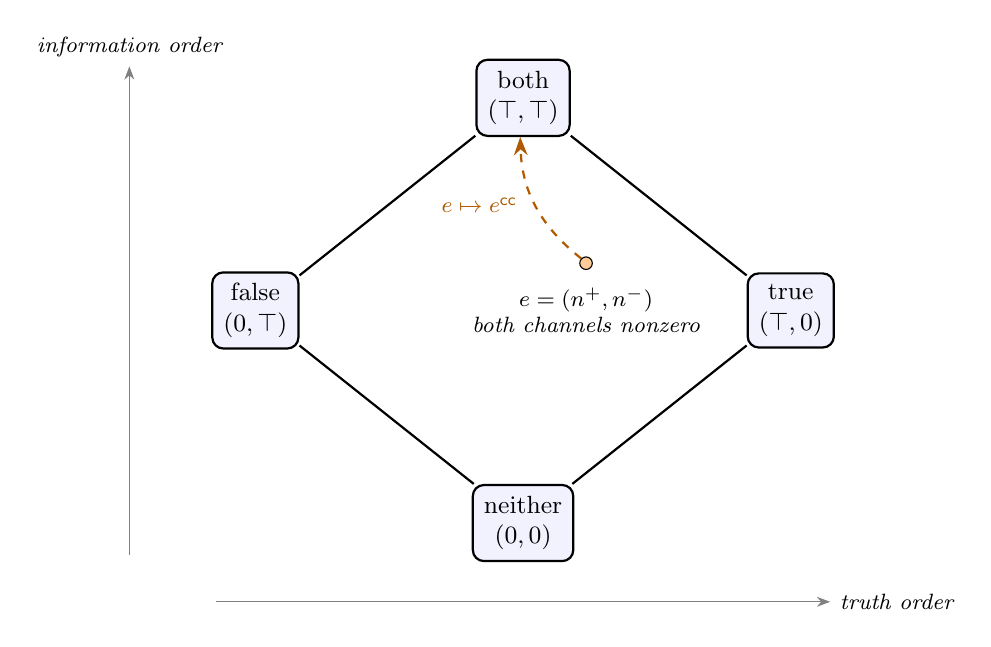
\begin{tikzpicture}[
  corner/.style={draw, rounded corners, thick, align=center, inner sep=4pt,
    font=\small, fill=blue!5},
  lab/.style={font=\footnotesize\itshape}]
\node[corner] (b) at (0,2.7) {both\\$(\top,\top)$};
\node[corner] (n) at (0,-2.7) {neither\\$(0,0)$};
\node[corner] (t) at (3.4,0) {true\\$(\top,0)$};
\node[corner] (f) at (-3.4,0) {false\\$(0,\top)$};
\draw[thick] (n) -- (t) -- (b) -- (f) -- (n);
\draw[-{Stealth}, gray] (-5.0,-3.1) -- (-5.0,3.1) node[lab, above, black]
  {information order};
\draw[-{Stealth}, gray] (-3.9,-3.7) -- (3.9,-3.7) node[lab, right, black] {truth order};
\node[draw, circle, fill=orange!40, inner sep=1.6pt] (e) at (0.8,0.6) {};
\node[lab, align=center, below=3pt of e] {$e=(n^+,n^-)$\\both channels nonzero};
\draw[-{Stealth}, orange!70!black, thick, dashed] (e) to[bend left=25]
  node[lab, left=3pt, pos=0.5] {$e\mapsto e^{\mathsf c\mathsf c}$} (b);
\end{tikzpicture}
\caption{The four corners of the catuṣkoṭi as Belnap's four values \cite{Belnap1977} inside
PLN evidence.
Vertically, the information order; horizontally, the truth order. Double negation sends
every evidence value to the corner whose channels it touches.}
\label{fig:corners}
\end{figure}

\subsection{FDE is the logic of support}

Say that a formula is \emph{supported} by an evidence valuation when its positive channel is
nonzero, and \emph{refuted} when its negative channel is. Interpret conjunction and
disjunction on the truth order and negation as the exchange of channels.

\begin{theorem}[The catuṣkoṭi is FDE over evidence]
For every valuation $v$ of atoms in $\BE$ and every formula $\varphi$, support and
refutation of $\varphi$ are exactly Dunn's four-valued evaluation \cite{Dunn1976} of
$\varphi$ at the supports of the atoms. Hence the logic of supported formulas over PLN evidence is FDE, and
magnitudes never affect satisfaction: they affect strength only.
\end{theorem}

\begin{lstlisting}
theorem support_refutation_evalEvidence (v : Atom → BinaryEvidence) :
    ∀ formula : AtomFormula Atom,
      ((evalEvidence v formula).pos ≠ 0 ↔ (atomSystem.eval (supportValuation v) formula).1) ∧
        ((evalEvidence v formula).neg ≠ 0 ↔ (atomSystem.eval (supportValuation v) formula).2)
\end{lstlisting}

\noindent Priest stipulates FDE for the catuṣkoṭi; here it is a theorem about a carrier the
library already uses for inference: FDE is the support-level shadow of PLN evidence.

\section{Two negations and the two tetralemmas}
\label{sec:negations}

\subsection{The doctrine}

Westerhoff explains why Nāgārjuna's tetralemma, which rejects a statement, its negation, both
and neither, is not simply inconsistent \cite[p.~28]{Westerhoff2007}:

\begin{quote}
Some are implicational negations (paryudāsapratiṣedha) which make an assertion about the
object referred to (`the apple is not red' implies that it is some other colour), while
others are non-implicational (prasajyapratiṣedha) and do not make such an assertion (`the
force of gravity is not red' does not imply that it is some other colour).
\end{quote}

\subsection{Strong and intuitionistic negation}

On the truth order of $\BE$ there are two negations. Strong negation $\sim a$, Nelson's
constructible falsity \cite{Nelson1949}, exchanges the channels: it asserts evidence against. Intuitionistic negation
$\mathrm{inot}\,a$ asserts only that there is no support. These are the implicational and
non-implicational negations respectively.

\begin{theorem}[When absence of support counts against]
Intuitionistic negation entails strong negation on the truth order exactly when the absence
of support is full refutation.
\end{theorem}

\begin{lstlisting}
theorem inot_truthLE_cdNeg_iff (a : BinaryEvidence) :
    TruthLE (inot a) (∼a) ↔ (a.pos = 0 → a.neg = ⊤)
\end{lstlisting}

\noindent This is already the PLN form of the non-perception rule of
Section~\ref{sec:nonperception}: ``no support'' may be booked as evidence against only where
the source is complete.

\subsection{The two extremes of the theory lattice}
\label{sec:extremes}

\begin{theorem}[Positive and negative tetralemma]
Over evidence valuations:
\begin{enumerate}
\item the theory of all formulas has as models exactly the valuations that give every atom
both support and refutation; there all four corners of every claim are supported;
\item exactly one valuation satisfies nothing, the one that is \emph{neither} at every atom;
there all four corners of every claim are unsupported, and all four are denied by
intuitionistic negation;
\item among consistent valuations, the theory of all formulas has no model.
\end{enumerate}
\end{theorem}

\begin{lstlisting}
theorem models_univ_eq_both :
    models (evidenceSat (Atom := Atom)) univ =
      {v | ∀ atom, (v atom).pos ≠ 0 ∧ (v atom).neg ≠ 0}
theorem corners_supported_of_degenerate {v : Atom → BinaryEvidence}
    (degenerate : Degenerate (evidenceSat (Atom := Atom)) v) (formula : AtomFormula Atom) :
    ∀ corner ∈ corners (evalEvidence v formula), Supported corner
theorem theoryOf_singleton_eq_empty_iff (v : Atom → BinaryEvidence) :
    theoryOf (evidenceSat (Atom := Atom)) {v} = ∅ ↔ v = neitherValuation
theorem corners_unsupported_at_neither (formula : AtomFormula Atom) :
    ∀ corner ∈ corners (evalEvidence (Atom := Atom) neitherValuation formula),
      ¬ Supported corner
theorem corners_denied_at_neither (formula : AtomFormula Atom) :
    ∀ corner ∈ corners (evalEvidence (Atom := Atom) neitherValuation formula),
      Supported (inot corner)
theorem modelsIn_consistent_univ_eq_empty [Nonempty Atom] :
    modelsIn (evidenceSat (Atom := Atom)) consistentValuations univ = ∅
\end{lstlisting}

\noindent Priest introduces a fifth value for ``none of the four'', because \emph{neither}
is itself one of the four \cite{Priest2018}; Kapsner questions whether that value can be one
more truth value of the same kind \cite{Kapsner2020}. On evidence the difficulty splits by negation: with the corners
stated using the presupposing (intuitionistic) negation, all four are denied at the
\emph{neither} valuation, consistently, without a fifth object-level value. What a fifth
value genuinely captures, an evaluation with no result at all, is a different kind of
``nothing'' and belongs with the kinds of Section~\ref{sec:novalue}.

\subsection{The liar's two escapes}

Garfield and Priest read Nāgārjuna's limit contradictions dialetheically
\cite{GarfieldPriest2003}; others read them as presupposition failures. In Kripke's theory of
truth \cite{Kripke1975} these are the two extreme fixed points of one monotone jump; when the
base facts are bivalent, conflation \cite{Fitting1989} exchanges them.

\begin{theorem}[Paracomplete and dialetheic readings are dual]
A judgment is undetermined in the least fixed point exactly when it both holds and fails in
the greatest; the liar is \emph{both} in the greatest fixed point.
\end{theorem}

\begin{lstlisting}
theorem undetermined_least_iff_both_greatest (judgment : Judgment) :
    (judgment ∉ system.least.holds ∧ judgment ∉ system.least.fails) ↔
      (judgment ∈ system.greatest.holds ∧ judgment ∈ system.greatest.fails)
theorem liar_both_greatest {liar : Judgment} (isLiar : system.spec liar = .neg (.truth liar)) :
    liar ∈ system.greatest.holds ∧ liar ∈ system.greatest.fails
\end{lstlisting}

\noindent The choice between the two readings is a choice of fixed point, not of foundations.

\section{Non-perception}
\label{sec:nonperception}

\subsection{The doctrine}

The \emph{Tarkabhāṣā} of Mokṣākaragupta, in Kajiyama's translation \cite{Kajiyama1966},
illustrates the logical mark of non-cognition (§13):

\begin{quote}
In this place there is no jar, because it is not cognized though it is by nature
perceptible.
\end{quote}

\noindent The qualifier carries the whole weight (§13.3):

\begin{quote}
\ldots the mere non-occurrence of cognition regarding objects which are inaccessible in
space, time and essence, does not establish practical activities referring to the negation
[of the object concerned]; such objects are illustrated by Mt.~Sumeru [which is spatially
inaccessible], the future emperor Śaṅkha [who is inaccessible in time] and a ghost [which is
inaccessible in essence].
\end{quote}

\noindent Kajiyama's note summarizes Dharmakīrti's two kinds of non-cognition: ``the former
leads to the result through the absence of the proof, while the latter through the presence
of the counter-proof; i.e.\ the former through doubt while the latter through the definite
knowledge of absence.'' And (§13.4): ``With regard to a future experience, however,
non-cognition is itself doubtful and accordingly cannot be a means of valid knowledge.''

Stcherbatsky explains what ``perceptible'' means for an absent thing, quoting Dharmottara
\cite[p.~365]{Stcherbatsky1932}:

\begin{quote}
The perception of an absent thing is impossible, it is a contradiction. If it is perception,
the thing is present, it cannot be absent. But how is it present? It is present in
imagination and that means that all the conditions necessary for its perception are
fulfilled. It would be necessarily perceived if it were present; but it is absent and
therefore it is only imagined, but not perceived, it is perceived in imagination. [\ldots]
«How is it possible for an object, say a jar, to be perceptible, when it is absent? It is
said to be perceptible, although it is absent, because its perceptibility is imagined! We
imagine it in the following way: ``If it were present on this spot, it certainly would have
been perceived''.»
\end{quote}

\subsection{The law}

\begin{definition}
A \emph{frame} is a set of stages $W$ with a reflexive relation $\mathrm{Future}$ and a
predicate $\mathrm{Perceived}$. At a stage $w$:
\begin{itemize}
\item the thing is \emph{absent} if no future stage perceives it;
\item the stage is \emph{perceptible} if whatever a future stage perceives is already
perceived at $w$;
\item the stage is \emph{in doubt} if the thing is neither perceived nor absent.
\end{itemize}
\end{definition}

\noindent Perceptibility is Dharmottara's counterfactual made exact: ``if it were present on
this spot, it certainly would have been perceived'' becomes ``whatever a later stage would
perceive is perceived already''.

\begin{lstlisting}
structure Frame (W : Type u) where
  Future : W → W → Prop
  future_refl : ∀ w, Future w w
  Perceived : W → Prop
def Absent (w : W) : Prop := ∀ w', F.Future w w' → ¬ F.Perceived w'
def Perceptible (w : W) : Prop := ∀ w', F.Future w w' → F.Perceived w' → F.Perceived w
def Doubt (w : W) : Prop := ¬ F.Perceived w ∧ ¬ F.Absent w
\end{lstlisting}

\begin{theorem}[Non-perception]
At a perceptible stage, absence is exactly non-perception. Perceptibility is exactly the
condition under which non-perception establishes absence. A stage is in doubt exactly when
it is not perceptible, and every stage is perceived, absent or in doubt.
\end{theorem}

\begin{lstlisting}
theorem absent_iff_not_perceived {w : W} (perceptible : F.Perceptible w) :
    F.Absent w ↔ ¬ F.Perceived w
theorem perceptible_iff {w : W} : F.Perceptible w ↔ (¬ F.Perceived w → F.Absent w)
theorem doubt_iff_not_perceptible {w : W} : F.Doubt w ↔ ¬ F.Perceptible w
theorem perceived_or_absent_or_doubt (w : W) :
    F.Perceived w ∨ F.Absent w ∨ F.Doubt w
\end{lstlisting}

\begin{figure}[ht]
\centering
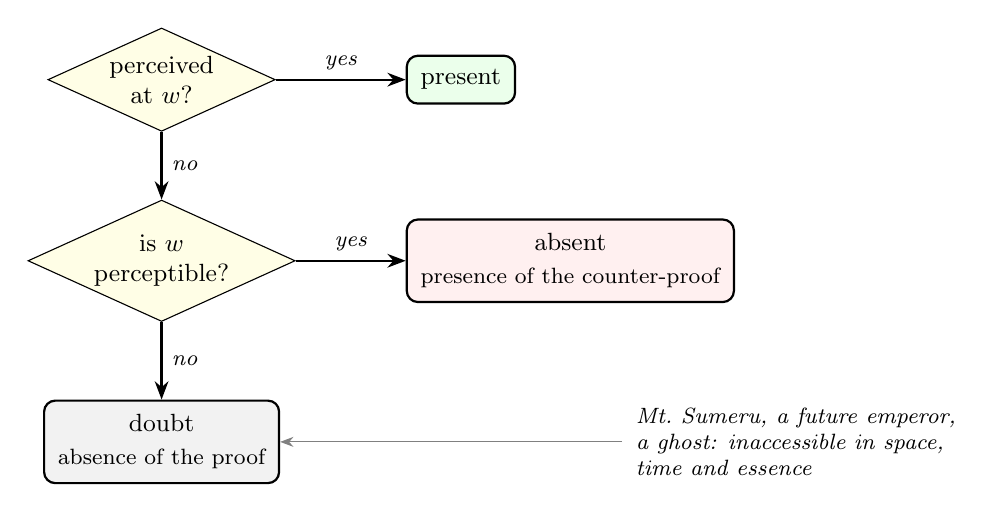
\begin{tikzpicture}[
  box/.style={draw, rounded corners, thick, align=center, font=\small, inner sep=5pt},
  q/.style={draw, diamond, aspect=2.2, align=center, font=\small, inner sep=1pt,
    fill=yellow!10},
  lab/.style={font=\footnotesize\itshape}]
\node[q] (p) at (0,0) {perceived\\at $w$?};
\node[box, fill=green!8, anchor=west] (pres) at (3.1,0) {present};
\node[q] (pc) at (0,-2.3) {is $w$\\perceptible?};
\node[box, fill=red!6, anchor=west] (abs) at (3.1,-2.3) {absent\\[1pt]
  {\footnotesize presence of the counter-proof}};
\node[box, fill=gray!10] (dbt) at (0,-4.6) {doubt\\[1pt]
  {\footnotesize absence of the proof}};
\draw[-{Stealth}, thick] (p) -- node[lab, above] {yes} (pres);
\draw[-{Stealth}, thick] (p) -- node[lab, right] {no} (pc);
\draw[-{Stealth}, thick] (pc) -- node[lab, above] {yes} (abs);
\draw[-{Stealth}, thick] (pc) -- node[lab, right] {no} (dbt);
\node[lab, align=left, anchor=west] at (5.9,-4.6)
  {Mt.~Sumeru, a future emperor,\\a ghost: inaccessible in space,\\time and essence};
\draw[-{Stealth}, gray] (5.85,-4.6) -- (dbt.east);
\end{tikzpicture}
\caption{The non-perception law. Not perceiving establishes absence only at a perceptible
stage; elsewhere it leaves doubt.}
\label{fig:nonperception}
\end{figure}

\subsection{Eight instances, and Chalmers's ``that's all''}

The same law appears in the library about eight times under other names, each with its own
reflection or completeness condition playing the role of perceptibility:
\begin{itemize}
\item absence in presheaf models of events;
\item permitted absence of reactions in a scoped process calculus;
\item refutation by a decision backend, which is allowed only when the backend is closed;
\item answers outside a decidable fragment;
\item fuel-bounded runs, where exhaustion is doubt and not refusal;
\item underfunded assays, which stay quiet in both directions;
\item scenario bases, through Chalmers's ``that's all'' clause;
\item concept construction at a vantage.
\end{itemize}
\noindent Each is re-derived from the law as a corollary. Two of them:

\begin{lstlisting}
theorem thatsAll_iff_perceptible (actual : S) :
    I.ThatsAll positive actual ↔
      ∀ sentence, (scenarioFrame I positive sentence).Perceptible actual
theorem exhaustedAsRefusal_books_doubt {logical : Query → Option Answer}
    {run : Query → Nat → RunOutcome Answer} {query : Query} {fuel : Nat} {answer : Answer}
    (exhausted : run query fuel = .exhausted) (answerable : logical query = some answer) :
    (runFrame logical run query fuel).Doubt false ∧
      exhaustedAsRefusal (run query fuel) = some none
\end{lstlisting}

\noindent The first is worth reading slowly. In Chalmers's scrutability base PQTI
\cite{Chalmers2012}, the ``that's all'' truth $T$ says that the world is no more than the
base truths require. The theorem says that $T$ holds at the actual scenario exactly when
every sentence is perceptible there. So $T$ is perceptibility made global: with it, what the
base does not contain is absent, and the world is closed; without it, the frontier beyond
the base stays in doubt, and the world is open. The closed world and the open-ended world
meet at exactly one clause.

\subsection{A rule for evidence}

The PLN consequence is a single bookkeeping rule. Absence of support may be booked as
negative evidence only for a proposition the source is complete for; otherwise it stays in
the \emph{neither} corner $(0,0)$. A certificate of exhaustion is itself positive evidence
(``the presence of the counter-proof''), which is why a completed search can refute while a
timed-out one cannot.

\section{Valid reasons}
\label{sec:reasons}

\subsection{The three marks}

The \emph{Tarkabhāṣā} (§10) states the triple characteristic of a logical mark $h$ for the
property $s$ of a subject $p$ \cite{Kajiyama1966}:

\begin{quote}
1) Its [h's] definite (niścitam) presence in all [the members of the class of] the locus
(p) of inference [as well as in other classes].\\
2) Its definite presence only in things similar to p [sapakṣa i.e.\ the members of the
class of s].\\
3) Its definite, absolute absence in the anti-pakṣa [vipakṣa i.e.\ any member of the class
incompatible with s].
\end{quote}

\noindent The second is named \emph{anvaya} (positive pervasion), the third \emph{vyatireka}
(negative pervasion).

\begin{theorem}[Soundness of the marks]
If the reason holds of the subject and is universally absent wherever the property is
absent, the property holds of the subject.
\end{theorem}

\begin{lstlisting}
theorem sound_of_marks {subject : α} {reason property : α → Prop} (paksha : reason subject)
    (vyatireka : ∀ x, ¬ property x → ¬ reason x) : property subject
\end{lstlisting}

\noindent Stcherbatsky adds a remark that the wheel below makes exact
\cite[p.~244]{Stcherbatsky1932}:

\begin{quote}
It is easily seen that the second and the third rule mutually imply each the other. If the
reason is present in the similar instances only, it also is absent from every dissimilar case.
And if it is absent from every dissimilar case, it can be present in similar instances only,
although not necessarily in all of them. Nevertheless both rules must be mentioned, because,
although in a correct inference the application of the one means the application of the
other, in a logical fallacy their infringements carry sometimes different results.
\end{quote}

\noindent The difficulty is the word ``absolute'': observed absence on examined cases is not
universal absence. The library makes the step from one to the other an instance of
non-perception.

\begin{theorem}[Induction is non-perception of a counterexample]
Form a two-stage frame whose stages are the examined instances and all instances, and which
perceives a counterexample when one is found. The examination is perceptible exactly when
every counterexample would have been examined; then observed exclusion is universal.
Otherwise an unexamined counterexample leaves the inference in doubt.
\end{theorem}

\begin{lstlisting}
theorem inductionFrame_perceptible_iff :
    (inductionFrame examined reason property).Perceptible false ↔
      ((∃ x, reason x ∧ ¬ property x) → ∃ x ∈ examined, reason x ∧ ¬ property x)
theorem universal_of_observed
    (perceptible : (inductionFrame examined reason property).Perceptible false)
    (observed : ∀ x ∈ examined, ¬ property x → ¬ reason x) :
    ∀ x, ¬ property x → ¬ reason x
theorem doubt_of_unexamined_counterexample
    (observed : ∀ x ∈ examined, ¬ property x → ¬ reason x)
    {c : α} (carries : reason c) (lacks : ¬ property c) :
    (inductionFrame examined reason property).Doubt false
\end{lstlisting}

\subsection{Dignāga's wheel of reasons}

Dignāga tabulated the possible positions of a reason by its presence among similar
instances (those with the property) and among dissimilar instances (those without it), each
``in all'', ``in some'' or ``in none''. Stcherbatsky describes the table
\cite[p.~321]{Stcherbatsky1932}:

\begin{quote}
All the possible positions of the reason between similar and dissimilar instances are
computed in this table, according to a mathematical principle. The result is that there are
only nine positions of the Reason, neither more, nor less. Of them two only represent right
reasons, the remaining seven are fallacies. Out of these seven, two represent the fallacy at
its maximum, they are the contradictorily opposed part of right reason, and are called
«contrary» or «inverted» reasons. The five remaining ones are «uncertain», because the
position of the middle term between similar and dissimilar instances is not definite;
[\ldots]
\end{quote}

\noindent Figure~\ref{fig:wheel} gives the table in the form the library uses. Of the five
uncertain positions, the library names the two extreme ones separately, as \emph{too wide}
(present everywhere) and \emph{too narrow} (present nowhere).

\begin{figure}[ht]
\centering
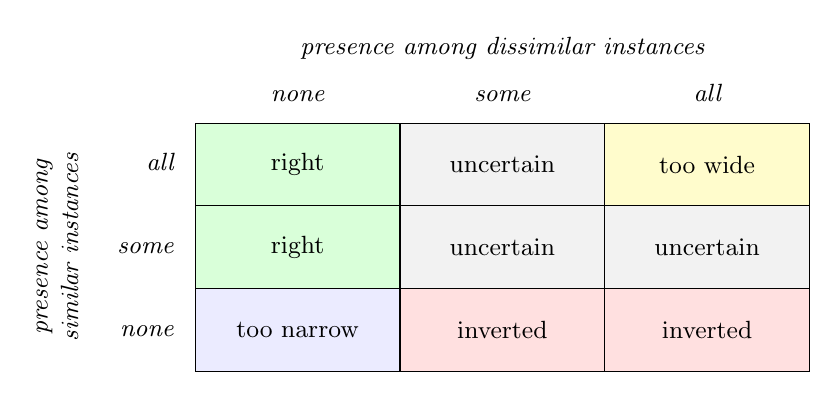
\begin{tikzpicture}[
  cell/.style={draw, minimum width=2.6cm, minimum height=1.05cm, align=center,
    font=\small},
  head/.style={font=\small\itshape, align=center}]
\def\cw{2.6}\def\ch{1.05}
\foreach \c/\txt in {0/none,1/some,2/all} {
  \node[head, anchor=base] at ({\c*\cw}, 0.8) {\txt};
}
\node[head, anchor=base] at ({1*\cw}, 1.4) {presence among dissimilar instances};
\foreach \r/\txt in {0/all,1/some,2/none} {
  \node[head, anchor=base east] at (-1.45, {-\r*\ch-0.08}) {\txt};
}
\node[head, rotate=90] at (-3.05, {-1*\ch}) {presence among\\similar instances};
% row all
\node[cell, fill=green!15] at (0,0) {right};
\node[cell, fill=gray!10] at (\cw,0) {uncertain};
\node[cell, fill=yellow!20] at ({2*\cw},0) {too wide};
% row some
\node[cell, fill=green!15] at (0,{-\ch}) {right};
\node[cell, fill=gray!10] at (\cw,{-\ch}) {uncertain};
\node[cell, fill=gray!10] at ({2*\cw},{-\ch}) {uncertain};
% row none
\node[cell, fill=blue!8] at (0,{-2*\ch}) {too narrow};
\node[cell, fill=red!12] at (\cw,{-2*\ch}) {inverted};
\node[cell, fill=red!12] at ({2*\cw},{-2*\ch}) {inverted};
\end{tikzpicture}
\caption{Dignāga's wheel as defined in the library: two right cells, two inverted, one too
wide, one too narrow and three uncertain. Reading presence among similar instances as
support and presence among dissimilar instances as refutation, \emph{right} is the
\emph{true} corner, \emph{inverted} the \emph{false} corner, \emph{too narrow} the
\emph{neither} corner, and \emph{too wide} and \emph{uncertain} are the \emph{both} corner.
The four cells built from ``all'' and ``none'' are the saturated corners of
Figure~\ref{fig:corners}; ``some'' is a magnitude that double negation forgets.}
\label{fig:wheel}
\end{figure}

\begin{lstlisting}
def wheel : Occurrence → Occurrence → WheelVerdict
  | .all, .all => .tooWide
  | .none, .all => .inverted
  | .some, .all => .uncertain
  | .all, .none => .right
  | .none, .none => .tooNarrow
  | .some, .none => .right
  | .all, .some => .uncertain
  | .none, .some => .inverted
  | .some, .some => .uncertain
theorem wheel_quadrant (similar dissimilar : Occurrence) :
    (wheel similar dissimilar).quadrant = supportQuadrant similar.present dissimilar.present
\end{lstlisting}

\begin{theorem}[The wheel is pervasion evidence]
Count the reason among the similar and among the dissimilar instances; this is the evidence
for the implication from reason to property. A reason is in a \emph{right} position exactly
when that evidence has strength $1$, and \emph{too narrow} exactly when there is no evidence at
all. For every nonzero prior, finite counts have confidence strictly below $1$.
\end{theorem}

\begin{lstlisting}
theorem wheelOf_right_iff_strength :
    wheelOf similar dissimilar reason = .right ↔
      (pervasionEvidence similar dissimilar reason).toStrength = 1
theorem wheelOf_tooNarrow_iff_total :
    wheelOf similar dissimilar reason = .tooNarrow ↔
      (pervasionEvidence similar dissimilar reason).total = 0
theorem pervasion_confidence_lt_one {κ : ENNReal} (prior : κ ≠ 0) :
    BinaryEvidence.toConfidence κ (pervasionEvidence similar dissimilar reason) < 1
\end{lstlisting}

\noindent Counting never certifies a pervasion. Nor does a right cell settle the subject,
which belongs to neither class: three instances already give a reason in a right cell whose
subject carries the reason and lacks the property (\lean{right_cell_not_conclusive}). In the
language of rule learning, a \emph{too narrow} reason, present only in the subject, is a rule
that covers nothing but its own training example: it carries no evidence at all.

\subsection{The three kinds of reason}

Dharmakīrti's \emph{Nyāyabindu} (II.19, quoted in the \emph{Tarkabhāṣā}) divides reasons
into three kinds: ``Among [the three kinds of logical marks] the two [i.e.\ the identical
and causal marks] are for establishing the existence of real entities, the other one [i.e.\
the mark of non-cognition] is the probans for negation.'' Each supplies the certificate of
pervasion that counting cannot.

The \emph{identity} (essence) mark is a reason whose concept entails the property's, so the
pervasion holds in every structure. Over evidence, a conjunction is an essence reason for each
of its conjuncts, and a disjunction is not one for its disjuncts.

\begin{lstlisting}
theorem essence_pervasion {reasonSentence propertySentence : Sent}
    (entails : Entails Sat {reasonSentence} propertySentence) (m : Str)
    (carries : Sat m reasonSentence) : Sat m propertySentence
theorem essence_conj (first second : AtomFormula Atom) :
    Entails evidenceSat {.conj first second} first
theorem not_essence_disj :
    ¬ Entails (evidenceSat (Atom := Bool)) {.disj (.truth true) (.truth false)} (.truth true)
\end{lstlisting}

\noindent The mark of non-cognition is the law of Section~\ref{sec:nonperception}, applied to
the counterexample as above. The \emph{causal} mark is proved over structural causal models,
with a control showing exactly when it fails.

\begin{lstlisting}
theorem effect_pervasion {mechanisms : Mechanisms Key Bool} {effect cause : Key}
    (requires : RequiresCause mechanisms effect cause) {store : Key → Bool}
    (solution : IsSolution mechanisms store) (seen : store effect = true) :
    store cause = true
theorem smokeMachine_breaks_pervasion :
    ¬ RequiresCause (surgery smokeMachine (mechanisms false)) .smoke .fire ∧
      machineSmoke .smoke = true ∧ machineSmoke .fire = false
\end{lstlisting}

\noindent If the mechanism of smoke produces it only where there is fire, every solution with
smoke has fire. Under the intervention that installs a smoke machine, smoke without fire is a
solution: the effect reason fails exactly when its mechanism is replaced.

\section{Meaning by exclusion}
\label{sec:apoha}

\subsection{The doctrine}

Katsura summarizes Dignāga's theory of meaning \cite{Katsura1979}:

\begin{quote}
In the Fifth Chapter of the P(ramāṇa)S(amuccaya) Dignāga presents the theory of anyāpoha
(exclusion of others) which may be regarded as his most original contribution to Indian
logic. Dignāga declares in the introductory verse (K.~1) that verbal cognition (śabda) is
nothing but inference (anumāna) because both of them function on the principle of
anyāpoha.
\end{quote}

\noindent Stcherbatsky states the thesis in its starkest form, reporting Śāntarakṣita and
Kamalaśīla \cite[p.~471]{Stcherbatsky1932}:

\begin{quote}
[\ldots] the words express their own meaning through negation. They are therefore negative.
Without negation they express nothing, they can express something only dialectically, i.e.
in couples of mutual negation.
\end{quote}

\subsection{Concepts as double exclusion}

Apoha relies on a dichotomy that Stcherbatsky's account of Dharmakīrti states as the law of
contradiction \cite[pp.~403 and 417]{Stcherbatsky1932}:

\begin{quote}
«There is contradiction, says he, in a couple whose essence is posited in a complete mutual
exclusion, as, e.g., existence and non-existence». Complete mutual exclusion means mutual
exclusion without anything intermediate.
\end{quote}

\begin{quote}
When we cognize a patch of blue in the judgment «this is blue», we then, owing to a Primordial
Function of Productive Imagination, construct out of the Universe of Discourse two parts, the
blue and the non-blue. Everything that is not referred to the blue will be necessarily in the
non-blue. There can be no third possibility, nothing in the middle.
\end{quote}

\noindent For an observer, exclusion is a symmetric irreflexive relation of witnessed
apartness. The exclusion of a class is everything apart from all of its members, and a
concept is a class equal to its double exclusion. These closed classes are the propositions
of Goldblatt's semantics for orthologic \cite{Goldblatt1974}.

\begin{theorem}[Apoha]
Treble exclusion is exclusion. Concepts by exclusion are exactly the extents of the exclusion
context. Nothing lies in a class and in its exclusion, and a class together with its exclusion
generates every instance. Yet every instance lies in each concept or in its exclusion exactly
when non-exclusion is transitive.
\end{theorem}

\begin{lstlisting}
theorem excluded_excluded_excluded (S : Set V) :
    excluded excludes (excluded excludes (excluded excludes S)) = excluded excludes S
theorem isConcept_iff_isExtent (S : Set V) : IsConcept excludes S ↔ Order.IsExtent excludes S
theorem inter_excluded_eq_empty (S : Set V) : S ∩ excluded excludes S = ∅
theorem exclusionClosure_union_excluded (S : Set V) :
    excluded excludes (excluded excludes (S ∪ excluded excludes S)) = univ
theorem union_excluded_eq_univ_iff :
    (∀ S, IsConcept excludes S → S ∪ excluded excludes S = univ) ↔
      ∀ x y z, ¬ excludes x y → ¬ excludes y z → ¬ excludes x z
-- control: three instances, the middle one indistinguishable from both ends
theorem middle_in_neither :
    (1 : Fin 3) ∉ ({0} : Set (Fin 3)) ∪ excluded tolerance.Apart {0}
\end{lstlisting}

\noindent The theorem separates the two halves of the quoted law. ``Nothing in the middle'' is
a law of construction: a concept and its exclusion together generate the whole universe of
discourse. It is not a law of particulars: a particular may fall between a concept and its
exclusion whenever indistinguishability is not transitive, as the middle of three instances
does when it is indistinguishable from both ends while the ends are apart. The blue and the
non-blue exhaust what can be constructed, not what can be seen. Exclusion is not resemblance.

\subsection{Perception, construction and the sorites}
\label{sec:sorites}

The distinction calculus \cite{GoertzelDCalc} takes distinction as primitive: an observer is a
graded similarity on its instances, reflexive and symmetric. Its author states where the
structure lies:

\begin{quote}
[\ldots] indistinguishability is reflexive and symmetric but not transitive, and the failure of
transitivity, the sorites, is where all the nontrivial structure lives.
\end{quote}

\noindent The previous theorem says the same from the other side: particulars fall between a
concept and its exclusion exactly when indistinguishability is not transitive. The two meet in the
closure of an observer, which identifies whatever a chain of indistinguishable steps connects.
Read the observer as perception and its closure as conceptual construction. Dharmakīrti's
dichotomy is then a law of the closure, and it fails for the observer exactly on the sorites.

\begin{theorem}[Construction removes the middle]
Let exclusion be symmetric and irreflexive, and let the \emph{constructed} exclusion separate two
instances when no chain of indistinguishable steps connects them.
\begin{enumerate}
\item A class and its exclusion cover everything exactly when the class is closed under
indistinguishability.
\item The concepts of the observer that have no middle are exactly the concepts of its
construction.
\item An instance in the middle of a concept is indistinguishable from a member and from an
excluded instance, which exclude each other: every middle is the middle of a sorites triple.
\end{enumerate}
\end{theorem}

\begin{lstlisting}
def constructed (excludes : V → V → Prop) (x y : V) : Prop :=
  ¬ Relation.EqvGen (fun a b => ¬ excludes a b) x y
theorem union_excluded_eq_univ_iff_saturated (S : Set V) :
    S ∪ excluded excludes S = univ ↔ Saturated excludes S
theorem noMiddle_concept_iff (irrefl : ∀ x, ¬ excludes x x) (S : Set V) :
    (IsConcept excludes S ∧ S ∪ excluded excludes S = univ) ↔
      IsConcept (constructed excludes) S
theorem middle_sorites {S : Set V} (concept : IsConcept excludes S) {y : V}
    (notIn : y ∉ S) (notOut : y ∉ excluded excludes S) :
    ∃ x ∈ S, ∃ z ∈ excluded excludes S, ¬ excludes x y ∧ ¬ excludes y z ∧ excludes x z
\end{lstlisting}

\noindent Graded observers sharpen the picture. Read a similarity at a level $s$, counting two
instances apart when their similarity is below $s$. The distinction calculus has two transitivity
classes: \emph{metric}, where distances obey the triangle inequality, and \emph{ultrametric},
where similarity across two steps is at least that of the weaker step.

\begin{theorem}[The dichotomy at every resolution]
Every concept at every level $s\in(0,1]$ has no middle exactly when the observer is ultrametric.
The metric law is not enough: a metric observer on three instances, with neighbours at similarity
$3/4$ and the ends at $1/2$, has a concept with a middle at level $3/4$.
\end{theorem}

\begin{lstlisting}
theorem noMiddle_all_levels_iff_ultrametric (a : Tolerance W R) :
    (∀ s : R, 0 < s → s ≤ 1 → ∀ S, IsConcept (a.LevelApart s) S →
        S ∪ excluded (a.LevelApart s) S = univ) ↔ a.Ultrametric
theorem metricTolerance_metric : metricTolerance.Metric
theorem metricTolerance_not_ultrametric : ¬ metricTolerance.Ultrametric
theorem metric_middle :
    IsConcept (metricTolerance.LevelApart (3 / 4)) {0} ∧
      (1 : Fin 3) ∉ ({0} : Set (Fin 3)) ∪ excluded (metricTolerance.LevelApart (3 / 4)) {0}
\end{lstlisting}

\noindent In the three-instance observer of the previous control, construction connects the two
ends through the middle and separates nothing; the concept $\{0\}$, which has a middle for the
observer, is not a concept of the construction. Construction buys the dichotomy by forgetting the
distinction between the ends.

\subsection{Learning by exclusion}

\noindent Learning from examples then takes the familiar form of version spaces
\cite{Mitchell1982}, with concepts by exclusion as the hypotheses.

\begin{theorem}[Version spaces of concepts]
A concept consistent with positive and negative examples exists exactly when every positive
example excludes every negative one. The consistent concepts are exactly those between the
concept generated by the positives and the exclusion of the negatives.
\end{theorem}

\begin{lstlisting}
theorem consistent_iff {pos neg S : Set V} :
    Consistent excludes pos neg S ↔
      IsConcept excludes S ∧ excluded excludes (excluded excludes pos) ⊆ S ∧
        S ⊆ excluded excludes neg
theorem exists_consistent_iff {pos neg : Set V} :
    (∃ S, Consistent excludes pos neg S) ↔ Separated excludes pos neg
\end{lstlisting}

\begin{figure}[ht]
\centering
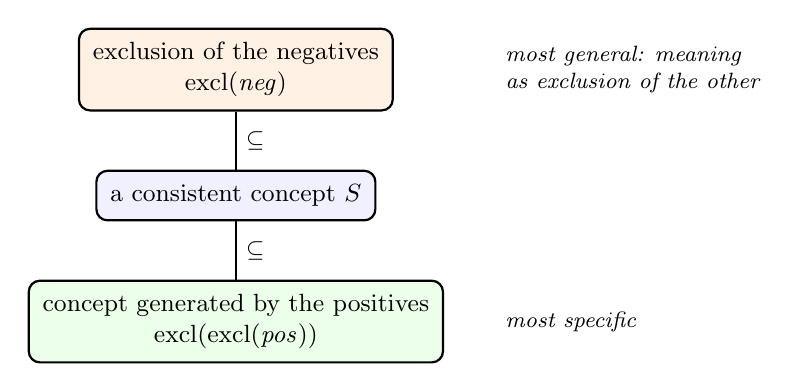
\begin{tikzpicture}[
  box/.style={draw, rounded corners, thick, align=center, font=\small, inner sep=5pt},
  lab/.style={font=\footnotesize\itshape}]
\node[box, fill=green!8] (spec) at (0,0) {concept generated by the positives\\
  $\mathrm{excl}(\mathrm{excl}(\mathit{pos}))$};
\node[box, fill=blue!6] (s) at (0,1.6) {a consistent concept $S$};
\node[box, fill=orange!10] (gen) at (0,3.2) {exclusion of the negatives\\
  $\mathrm{excl}(\mathit{neg})$};
\draw[thick] (spec) -- node[lab, right] {$\subseteq$} (s);
\draw[thick] (s) -- node[lab, right] {$\subseteq$} (gen);
\node[lab, align=left, anchor=west] at (3.3,0) {most specific};
\node[lab, align=left, anchor=west] at (3.3,3.2) {most general: meaning\\
  as exclusion of the other};
\end{tikzpicture}
\caption{The consistent hypotheses of learning by exclusion form an interval of concepts.}
\label{fig:apoha}
\end{figure}

\noindent A small example shows the interval. On a circle of six hues where each hue is
indistinguishable from its two neighbours, the observer has no metric law: $0$ and $2$ are
apart, though each is indistinguishable from $1$. The concept of $0$ is $\{0\}$, while its
resemblance class is $\{0,1,5\}$. From the positive example $0$ and the negative example $3$,
the consistent hypotheses are exactly four, from the concept of $0$ up to its resemblance
class:

\begin{lstlisting}
-- the six-hue circle
theorem conceptOf_zero : conceptOf hues.Apart 0 = {0}
theorem resemblance_zero : {y | ¬ hues.Apart 0 y} = {0, 1, 5}
theorem consistent_iff (S : Set (Fin 6)) :
    Consistent hues.Apart {0} {3} S ↔ S = {0} ∨ S = {0, 1} ∨ S = {0, 5} ∨ S = {0, 1, 5}
\end{lstlisting}

An experiment over random observers illustrates the point in numbers
(Table~\ref{tab:apoha}). Each row draws $200$ observers on $n$ instances, in which two
distinct instances are indistinguishable with probability $p$, and asks how concepts compare
with resemblance. For learning, each observer contributes one target concept with a middle;
half of its members, chosen at random, are the positive examples, and half of a pool, chosen
at random, are the negative examples. The pool is either the exclusion of the target or its
complement.

\begin{table}[ht]
\centering
\small
\setlength{\tabcolsep}{4pt}
\begin{tabular}{@{}lcc cccc cccc@{}}
\toprule
 & & & \multicolumn{4}{c}{negatives from the exclusion} &
  \multicolumn{4}{c}{negatives from the complement}\\
\cmidrule(lr){4-7}\cmidrule(l){8-11}
$n,\ p$ & concept $\subsetneq$ & middle & cons. & spec. & gen. & size &
  cons. & spec. & gen. & size\\
\midrule
8, 0.3 & 86.6\% & 92.6\% & 100\% & 8\% & 31\% & 5.4 & 56.5\% & 7\% & 29\% & 3.1\\
8, 0.5 & 98.1\% & 99.0\% & 100\% & 18\% & 46\% & 3.4 & 28.5\% & 5\% & 21\% & 1.6\\
10, 0.3 & 94.4\% & 98.0\% & 100\% & 9\% & 19\% & 7.1 & 34.5\% & 4\% & 23\% & 3.1\\
10, 0.5 & 99.6\% & 99.9\% & 100\% & 13\% & 35\% & 4.3 & 15.0\% & 7\% & 27\% & 1.7\\
\bottomrule
\end{tabular}
\caption{Learning by exclusion on random observers. \emph{concept $\subsetneq$}: the concept
of an instance is strictly inside its resemblance class. \emph{middle}: a proper concept has
instances in neither it nor its exclusion. \emph{cons.}: a consistent hypothesis exists.
Among the cases where one exists, \emph{spec.} and \emph{gen.}: the most specific or the most
general hypothesis is the target; \emph{size}: the mean number of consistent hypotheses.}
\label{tab:apoha}
\end{table}

\noindent Exclusion is almost never resemblance, and almost every concept has a middle.
Negative examples taken from what a concept excludes always admit a consistent hypothesis, as
the theorem requires; negative examples taken from mere non-membership fail to in $43$--$85\%$
of cases. ``Not a cow'' must be learned as ``excluded by cow'', not as ``not observed to be a
cow''. Where a hypothesis exists, the most general one, meaning as exclusion of the other,
recovers the target between two and six times as often as the most specific.

\section{The two truths}
\label{sec:twotruths}

\subsection{The doctrine}

Garfield and Priest present Nāgārjuna's doctrine \cite{GarfieldPriest2003}:

\begin{quote}
Central to Nagarjuna's view is his doctrine of the two realities. There is, according to
Nagarjuna, conventional reality and ultimate reality. Correspondingly, there are two truths:
conventional truth, that is, the truth about conventional reality, and ultimate truth, or the
truth about the ultimate reality---qua ultimate reality.
\end{quote}

\noindent They cite the verse that forbids taking emptiness itself as a view
(\emph{Mūlamadhyamakakārikā} XIII.8, Garfield's translation):

\begin{quote}
The Victorious ones have said\\
That Emptiness is the relinquishing of all views.\\
For whomever emptiness becomes a view\\
That one will accomplish nothing.
\end{quote}

\subsection{Madhyamaka: conventions carve the ultimate}

Fix a universe $U$ of structures and a theory $T$. A \emph{convention} $\Phi$ carves $U$ to the
structures satisfying $\Phi$. The \emph{conventional} truths under $\Phi$ are the
consequences of $T$ in the carved universe, and the \emph{ultimate} truths are the consequences
of $T$ in $U$ itself.

\begin{theorem}[Two truths as layering]
Every ultimate truth holds under every convention, and a conventional truth is an ultimate
truth of the enlarged theory: a convention is a commitment, not a fact. When conventions
cover the universe, the ultimate is their common part. Two disagreeing conventions, each with
a model, make neither of their claims ultimate.
\end{theorem}

\begin{lstlisting}
theorem ultimate_subset_conventional (U : Set Str) (Φ T : Set Sent) :
    ultimate Sat U T ⊆ conventional Sat U Φ T
theorem conventional_eq_ultimate (U : Set Str) (Φ T : Set Sent) :
    conventional Sat U Φ T = ultimate Sat U (Φ ∪ T)
theorem ultimate_eq_iInter_of_covers {ι : Sort uι} {U : Set Str} {conventions : ι → Set Sent}
    (covers : Covers Sat U conventions) (T : Set Sent) :
    ultimate Sat U T = ⋂ i, conventional Sat U (conventions i) T
theorem not_mem_ultimate_of_disagree {U : Set Str} {Φ Ψ T : Set Sent} {φ ψ : Sent}
    (holdsΦ : φ ∈ conventional Sat U Φ T) (holdsΨ : ψ ∈ conventional Sat U Ψ T)
    (hostedΦ : (modelsIn Sat (carve Sat U Φ) T).Nonempty)
    (hostedΨ : (modelsIn Sat (carve Sat U Ψ) T).Nonempty)
    (incompatible : ∀ m ∈ U, Sat m φ → Sat m ψ → False) :
    φ ∉ ultimate Sat U T ∧ ψ ∉ ultimate Sat U T
\end{lstlisting}

\begin{figure}[ht]
\centering
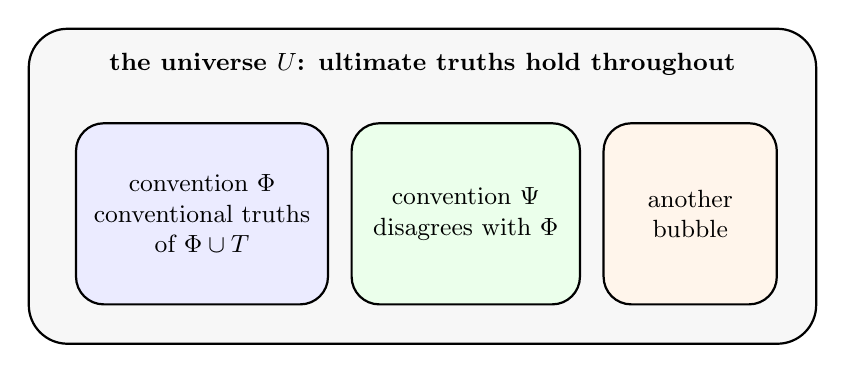
\begin{tikzpicture}[lab/.style={font=\footnotesize\itshape}]
\draw[thick, rounded corners=14pt, fill=gray!6] (-5,-1.9) rectangle (5,2.1);
\node[font=\small\bfseries] at (0,1.65) {the universe $U$: ultimate truths hold throughout};
\draw[thick, rounded corners=10pt, fill=blue!8] (-4.4,-1.4) rectangle (-1.2,0.9);
\node[align=center, font=\small] at (-2.8,-0.25) {convention $\Phi$\\
  conventional truths\\of $\Phi\cup T$};
\draw[thick, rounded corners=10pt, fill=green!8] (-0.9,-1.4) rectangle (2.0,0.9);
\node[align=center, font=\small] at (0.55,-0.25) {convention $\Psi$\\
  disagrees with $\Phi$};
\draw[thick, rounded corners=10pt, fill=orange!8] (2.3,-1.4) rectangle (4.5,0.9);
\node[align=center, font=\small] at (3.4,-0.25) {another\\bubble};
\end{tikzpicture}
\caption{Madhyamaka's two truths as the bubble/top layering. Conventions carve bubbles in the
universe; what holds throughout the universe holds in every bubble, while a bubble's truths
lift only as commitments.}
\label{fig:twotruths}
\end{figure}

\noindent This is the layering a type theory with local definitional equalities needs: each
bubble is a convention carving the ambient universe, what the top establishes holds in every
bubble, and a bubble's equalities never silently become global. The empty convention carves
nothing away, so its conventional truths are exactly the ultimate ones.

Over evidence the extremes of Section~\ref{sec:extremes} complete the picture. The theory of
all formulas has no consistent model: no consistent standpoint holds every view. At the other
extreme exactly one valuation holds no view at all, the one that is \emph{neither} at every
atom, and it satisfies no nonempty convention. So a family of conventions covers all evidence
only if one of them is the empty convention:

\begin{lstlisting}
theorem conventional_empty (U : Set Str) (T : Set Sent) :
    conventional Sat U ∅ T = ultimate Sat U T
theorem exists_empty_of_covers_univ {ι : Sort*} {conventions : ι → Set (AtomFormula Atom)}
    (covers : Covers evidenceSat univ conventions) : ∃ i, conventions i = ∅
\end{lstlisting}

\noindent Read against \emph{Mūlamadhyamakakārikā} XIII.8, the standpoint that relinquishes
all views is reached by no view; it is a point of the space of standpoints, not one more
theory in it. The two truths need it: without the empty convention, the conventions never
exhaust what evidence can be.

\subsection{Dharmakīrti: particulars and universals}

Dharmakīrti's two realities are a different structure. Stcherbatsky's section ``Two
realities'' opens with the definition \cite[p.~69]{Stcherbatsky1932}:

\begin{quote}
Existence, real existence, ultimate existence is nothing but efficiency. Whatsoever is
causally efficient is real. The non-efficient is unreal, it is a fiction. [\ldots] Only the
present, the «here», the «now», the «this» are real.
\end{quote}

\noindent The ultimately real is the particular, a structure; the conventionally real is the
universal, a class of structures. This is the
theory--model Galois connection, and over evidence it has a sharp consequence: two valuations
that satisfy exactly the same formulas, so that no concept separates them, can still differ
in strength.

\begin{lstlisting}
theorem no_concept_separates {K : Set (Atom → BinaryEvidence)}
    (extent : Order.IsExtent evidenceSat K) (member : leaning ∈ K) : doubting ∈ K
theorem strength_leaning_ne_doubting (atom : Atom) :
    (leaning atom).toStrength ≠ (doubting atom).toStrength
\end{lstlisting}

\noindent Here \code{leaning} gives every atom evidence $(2,1)$ and \code{doubting} gives
$(1,2)$: the same corner, strengths $2/3$ and $1/3$. What evidence does in inference, its
efficacy, Dharmakīrti's mark of the real, is finer than any concept of it.

\section{Kinds of ``no value''}
\label{sec:novalue}

A recurring source of trouble in programming languages is that distinct kinds of ``no value''
are collapsed into one: a missing result, an error, an unevaluated call, an explicit
\code{None}, an undetermined judgment, a refutation, an empty type. The precision about
absence that the previous sections formalize applies directly.

\subsection{Thirteen kinds, kept apart}

The library lists thirteen kinds, each with a witness on its own carrier, and proves that
every two kinds are separated by an observation.

\begin{lstlisting}
inductive Kind where
  | zeroAnswers | unitDatum | emptyCollection | errorValue | inertCall | noneValue
  | emptyDatum | neither | undetermined | incomplete | refuted
  | closedEmptyType | openDeclaredType
theorem Kind.separated {k k' : Kind} (different : k ≠ k') :
    ∃ observe : Witness → Prop, observe k.witness ∧ ¬ observe k'.witness
\end{lstlisting}

\noindent One collapse is instructive because it is also a cost. An evaluator that erases
error alternatives whenever a sibling alternative succeeds identifies kinds the list keeps
apart, and the rule is not monotone in the alternatives, so no producer that emits results as
they arrive can compute it: every level of evaluation must buffer.

\begin{lstlisting}
theorem heNormalize_not_monotone :
    ¬ ∀ bag bag' : Multiset Pattern, bag ≤ bag' → heNormalize bag ≤ heNormalize bag'
theorem no_streaming_heNormalize (emit : Multiset Pattern → Multiset Pattern)
    (monotone : ∀ bag bag', bag ≤ bag' → emit bag ≤ emit bag') :
    ¬ ∀ bag, emit bag = heNormalize bag
\end{lstlisting}

\subsection{Declared without constructors}

A type declared without constructors is not an empty type. Its theory is the theory of an
arbitrary set, possibly empty; adding a constructor later is conservative exactly when one
already exists; and only \emph{closing} the declaration, stating that these are all the
constructors, makes non-membership of other names refutable.

\begin{lstlisting}
theorem models_openDecl_empty : models (Sat (V := V)) (openDecl (∅ : Set N)) = univ
theorem conservative_iff (point : V) (ns : Set N) (d : N) :
    (∀ φ : Sentence N, Avoids d φ →
        Entails (Sat (V := V)) (openDecl (insert d ns)) φ →
          Entails (Sat (V := V)) (openDecl ns) φ) ↔ ns.Nonempty
theorem open_mem_undetermined {ns : Set N} {d : N} (fresh : d ∉ ns) {a b : V} (apart : a ≠ b) :
    Consistent (Sat (V := V)) (insert (.mem d) (openDecl ns ∪ distinctFrom d ns)) ∧
      Consistent (Sat (V := V)) (insert (.nonMem d) (openDecl ns ∪ distinctFrom d ns))
theorem closed_refutes_mem {ns : Set N} {d : N} :
    Entails (Sat (V := V)) (closedDecl ns ∪ distinctFrom d ns) (.nonMem d)
\end{lstlisting}

\noindent The open declaration is the non-perception law once more: before closing, membership
of a new name is in doubt; closing makes the declaration perceptible.

\subsection{Empty functions}

Sets and types answer one classic question differently. Functions out of the empty set into
any two codomains form one and the same set. As types, the function types out of the empty
type are only equivalent, one for each codomain.

\begin{lstlisting}
theorem funs_empty_eq (y y' : ZFSet.{u}) : ZFSet.funs ∅ y = ZFSet.funs ∅ y'
def emptyFunctionsEquiv (α β : Sort*) : (Empty → α) ≃ (Empty → β)
\end{lstlisting}

\subsection{Parameterized nulls}

A family of null values indexed by their kind can be handled by kind or uniformly. The
uniform view keeps the kind, re-raising an uncaught null keeps its kind and reason, and a null
at every proposition is inconsistent, which is why such nulls may live only in computational
types and never in propositions.

\begin{lstlisting}
theorem null_forget_kind {k : Kind} (n : Null k) :
    (Lifted.null n.forget : Lifted T).kindOf? = some k
theorem tryCatch_reraise_kind (n : AnyNull) (clauses : List (Clause T))
    (uncaught : ∀ clause ∈ clauses, clause.catches n = false) :
    (tryCatch (.null n) clauses).kindOf? = some n.1
theorem null_at_every_proposition_inconsistent (nullAt : ∀ P : Prop, P) : False
\end{lstlisting}

\section{What this offers reasoning systems}

The techniques the doctrines unify are known, and the honest claim is not that they are new.
Local closed-world reasoning, coverage scoring of candidate rules and paraconsistency each
exist on their own. What the Buddhist presentation adds is one law with an exact side
condition, and with it a way to state these techniques as instances of one principle instead
of as separate rules of thumb. Concretely:
\begin{itemize}
\item \textbf{Evidence chaining.} A chainer over PLN evidence may convert absence of support
into negative evidence only where the source is certified complete for the proposition
(Section~\ref{sec:nonperception}). Blanket closed-world rules, which treat ``nothing found''
as ``evidence against'', miscalibrate strength wherever the source is incomplete.
\item \textbf{Rule learning.} A candidate rule's position on the wheel is its coverage evidence
(Figure~\ref{fig:wheel}). A \emph{too narrow} rule carries no evidence; negative examples must
be certified exclusions, not mere non-memberships.
\item \textbf{Saturation-based proving.} ``Not derived, therefore not entailed'' is valid only
after a complete saturation; an interrupted run is doubt, never refusal.
\item \textbf{Conflicting knowledge.} First Degree Entailment over evidence lets a chainer carry
contradictory support, the \emph{both} corner, without explosion.
\end{itemize}
A demonstration would run a PLN chainer whose closed-world steps carry completeness
certificates, score rule candidates on the wheel, and keep \emph{both} as a value, measuring
calibration on knowledge bases with known gaps against blanket negation as failure.

\section{Conclusion}

The tradition's central move is to make the condition under which a negative inference holds
explicit: perceptibility for non-perception, absolute absence for the third mark, exclusion
rather than resemblance for concepts, conventions as commitments for truth. Each condition
becomes a hypothesis of a theorem, and each theorem comes with a control showing what goes
wrong without it. The result is less a new logic than a gain in semantic clarity: several
familiar techniques become instances of a few laws, and the laws state exactly when they
apply.

Readings of the texts are interpretations; the theorems are about the formal readings.

\appendix
\section{Modules and axioms}
\label{app:modules}

Every declaration quoted in this paper is proved in Lean~4 in the Mettapedia library, in the
modules below. An audit of all eighty declarations quoted or named in the text finds no
\code{sorry}. Twenty-two depend on no axiom at all; the others depend on at most Lean's
three standard axioms, \code{propext}, \code{Classical.choice} and \code{Quot.sound}.

\begin{center}
\small
\begin{tabular}{@{}ll@{}}
\toprule
Section & Module\\
\midrule
\ref{sec:corners}, \ref{sec:negations}, \ref{sec:reasons}, \ref{sec:twotruths} &
\lean{Mettapedia.PLN.RuleFamilies.QuantaleSemantics.DoubleNegationCorners}\\
 & \lean{Mettapedia.PLN.RuleFamilies.QuantaleSemantics.Tetralemma}\\
\ref{sec:negations} & \lean{Mettapedia.PLN.RuleFamilies.QuantaleSemantics.TwistNegation}\\
 & \lean{Mettapedia.GSLT.Logic.KripkeFixedPoint}\\
\ref{sec:nonperception} & \lean{Mettapedia.Logic.NonPerception}\\
 & \lean{Mettapedia.Logic.NonPerception.Instances}\\
\ref{sec:reasons} & \lean{Mettapedia.PLN.RuleFamilies.QuantaleSemantics.ReasonValidity}\\
\ref{sec:apoha} & \lean{Mettapedia.Cybernetics.DistinctionCalculus.Exclusion}\\
 & \lean{Mettapedia.Cybernetics.DistinctionCalculus.ExclusionLearning}\\
 & \lean{Mettapedia.Cybernetics.DistinctionCalculus.ConstructionMiddle}\\
\ref{sec:twotruths} & \lean{Mettapedia.Logic.TheoryModel.TwoTruths}\\
\ref{sec:novalue} & \lean{Mettapedia.Languages.MeTTa.Experimental.NoValueZoo}\\
 & \lean{Mettapedia.Logic.TheoryModel.OpenDeclarations}\\
 & \lean{Mettapedia.SetTheory.ZFSet.EmptyFunctions}\\
 & \lean{Mettapedia.Languages.MeTTa.Experimental.NullDesigns}\\
\bottomrule
\end{tabular}
\end{center}

\begin{thebibliography}{99}
\bibitem{Kajiyama1966} Y.~Kajiyama. \emph{An Introduction to Buddhist Philosophy: An Annotated
Translation of the Tarkabhāṣā of Mokṣākaragupta.} Memoirs of the Faculty of Letters, Kyoto
University, 10, 1966.
\bibitem{Priest2010} G.~Priest. The logic of the catuskoti. \emph{Comparative Philosophy}
1(2):24--54, 2010.
\bibitem{GarfieldPriest2003} J.~L.~Garfield and G.~Priest. Nāgārjuna and the limits of thought.
\emph{Philosophy East and West} 53(1):1--21, 2003.
\bibitem{Westerhoff2007} J.~Westerhoff. \emph{Nāgārjuna's Madhyamaka: A Philosophical
Investigation.} PhD thesis, School of Oriental and African Studies, University of London,
2007. Book version: \emph{Nāgārjuna's Madhyamaka: A Philosophical Introduction}, Oxford
University Press, 2009.
\bibitem{Katsura1979} S.~Katsura. The apoha theory of Dignāga. \emph{Journal of Indian and
Buddhist Studies (Indogaku Bukkyōgaku Kenkyū)} 28(1):489--493, 1979.
\bibitem{Priest2018} G.~Priest. \emph{The Fifth Corner of Four: An Essay on Buddhist
Metaphysics and the Catuṣkoṭi.} Oxford University Press, 2018.
\bibitem{Kapsner2020} A.~Kapsner. Cutting corners: a critical note on Priest's five-valued
catuṣkoṭi. \emph{Comparative Philosophy} 11(2):157--173, 2020.
\bibitem{Kripke1975} S.~Kripke. Outline of a theory of truth. \emph{Journal of Philosophy}
72(19):690--716, 1975.
\bibitem{Chalmers2012} D.~J.~Chalmers. \emph{Constructing the World.} Oxford University
Press, 2012.
\bibitem{Stcherbatsky1932} Th.~Stcherbatsky. \emph{Buddhist Logic}, vol.~1. Bibliotheca
Buddhica XXVI, part I, Academy of Sciences of the USSR, Leningrad, 1932. Corrected
republication, Dover, New York, 1962; page numbers as there.
\bibitem{Goldblatt1974} R.~Goldblatt. Semantic analysis of orthologic. \emph{Journal of
Philosophical Logic} 3:19--35, 1974.
\bibitem{Belnap1977} N.~D.~Belnap. A useful four-valued logic. In \emph{Modern Uses of
Multiple-Valued Logic}, Reidel, 1977, 5--37.
\bibitem{Dunn1976} J.~M.~Dunn. Intuitive semantics for first-degree entailments and ``coupled
trees''. \emph{Philosophical Studies} 29:149--168, 1976.
\bibitem{Nelson1949} D.~Nelson. Constructible falsity. \emph{Journal of Symbolic Logic}
14:16--26, 1949.
\bibitem{Fitting1989} M.~Fitting. Bilattices and the theory of truth. \emph{Journal of
Philosophical Logic} 18:225--256, 1989.
\bibitem{GoertzelDCalc} B.~Goertzel. The distinction calculus. Manuscript, corrected
September 2026.
\bibitem{Mitchell1982} T.~M.~Mitchell. Generalization as search. \emph{Artificial
Intelligence} 18:203--226, 1982.
\end{thebibliography}

\end{document}
